\textbf{Pour cette première partie, aucune justification n'est demandée et une seule réponse est possible par question. Pour chaque question, reportez son numéro sur votre copie et indiquez votre réponse.}

Une réponse fausse ou l'absence de réponse n'enlève aucun point.

\subsection*{Question 1}
Donner une écriture du nombre 0,75 sous la forme d'une fraction.

\subsection*{Question 2}
Calculer la somme \quad $-4,7 + 3,5$.

\subsection*{Question 3}
\begin{minipage}{0.6\linewidth}
	On considère le tableau de proportionnalité ci-contre.

	Combien vaut $a$ ?
\end{minipage}
\hfill
\begin{tblr}{hlines, vlines, colspec={X[2cm,c]X[2cm,c]}}
		6 & 18 \\
		12 & $a$ \\
\end{tblr}
\hfill~

\subsection*{Question 4}
Un sac contient 10 boules rouges, 4 boules bleues et 6 boules vertes.

On tire au hasard une boule dans le sac et on note sa couleur.

Sachant que toutes les boules ont la même probabilité d'être choisies, quelle est la probabilité d'obtenir une boule bleue?

\medskip
\begin{tblr}{colspec = {*4{X[c]}}}
	\textbf{A.}\quad $\dfrac{1}{4}$	 &
	\textbf{B.}\quad $\dfrac{4}{20}$ &
	\textbf{C.}\quad $\dfrac{4}{16}$ &
	\textbf{D.}\quad $\dfrac{1}{3}$	\\
\end{tblr}

\subsection*{Question 5}
Parmi les propositions suivantes, laquelle est la solution de l'équation \quad $10 x+16=-64$ ?

\medskip
\begin{tblr}{colspec = {*4{X[c]}}}
	\textbf{A.}\quad 8 &
	\textbf{B.}\quad $-4,8$&
	\textbf{C.}\quad $-8$ &
	\textbf{D.}\quad $-14$\\
\end{tblr}

\subsection*{Question 6}
Parmi les propositions suivantes, laquelle est la notation scientifique du nombre \np{0,00458} ?

\medskip
\begin{tblr}{colspec = {*4{X[c]}}}
	\textbf{A.}\quad $458 \times 10^{-3}$ &
	\textbf{B.}\quad $4,58 \times 10^{3}$ &
	\textbf{C.}\quad $4,58 \times 10^{-3}$&
	\textbf{D.}\quad $458 \times 10^{-5}$ \\
\end{tblr}

\subsection*{Question 7}
\begin{minipage}{0.6\linewidth}
	Le diagramme circulaire ci-contre donne la répartition des réponses de 24 élèves à une question à choix multiple.

	Quel est le nombre d'élèves ayant choisi la réponse B ?
\end{minipage}
\hfill~
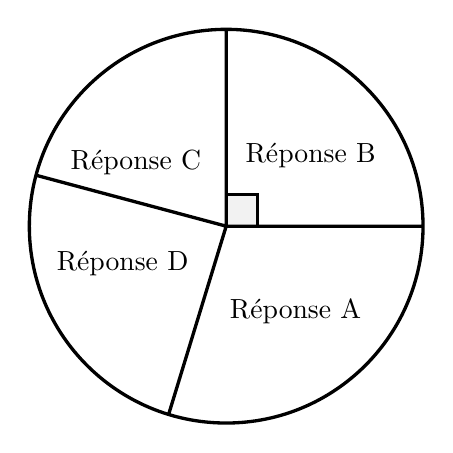
\begin{tikzpicture}[baseline={(0,0)}]
	\draw[line width=1pt, fill=gray!10] (0,0) rectangle (0.4,0.4) ;
	\draw[line width=1.2pt] (0,0)circle (2.5)
		(0,0)--(0:2.5)
		(0,0)--(-107:2.5)
		(0,0)--(90:2.5)
		(0,0)--(165:2.5);
	\node at (-51:1.4) {Réponse A};
	\node at (40:1.4) {Réponse B};
	\node at (145:1.4) {Réponse C};
	\node at (200:1.4) {Réponse D};
\end{tikzpicture}
\hfill~

\subsection*{Question 8}
\begin{minipage}{0.5\linewidth}
	Parmi les propositions suivantes, laquelle est le périmètre de la figure ci-contre?

\medskip
\begin{tblr}{colspec = {*2{X[c]}}}
	\textbf{A.}\quad \np[mm]{30}   &
	\textbf{B.}\quad \np[mm^2]{30} \\
 	\textbf{C.}\quad \np[mm]{50}   &
 	\textbf{D.}\quad \np[mm^2]{50} \\
 \end{tblr}
\end{minipage}
 \hfill~
 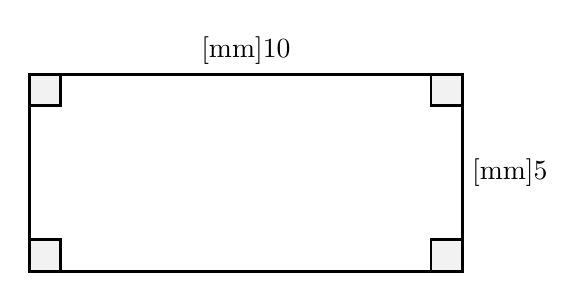
\begin{tikzpicture}[baseline={(0,1.25)}]
 	\draw[line width=1pt, fill=gray!10] (0,0) rectangle ++(0.4,0.4) ;
 	\draw[line width=1pt, fill=gray!10] (0,2.1) rectangle ++(0.4,0.4) ;
 	\draw[line width=1pt, fill=gray!10] (5.1,0) rectangle ++(0.4,0.4) ;
 	\draw[line width=1pt, fill=gray!10] (5.1,2.1) rectangle ++(0.4,0.4) ;
 	\draw[line width=1.2pt] (0,0) rectangle (5.5,2.5);
 	\node[above] at (2.75,2.5) {\np[mm]{10}};
 	\node[right] at (5.5,1.25) {\np[mm]{5}};
 \end{tikzpicture}
 \hfill~

\subsection*{Question 9}
Parmi les propositions suivantes, laquelle donne le cosinus de l'angle $\widehat{\mathrm{EDF}}$ dans le triangle rectangle ci-dessous ?

\medskip
\begin{tblr}{colspec = {*4{X[c]}}}
	\textbf{A.}\quad $\dfrac{4}{5}$&
	\textbf{B.}\quad $\dfrac{3}{5}$&
	\textbf{C.}\quad $\dfrac{5}{3}$&
	\textbf{D.}\quad $\dfrac{4}{3}$\\
\end{tblr}

\begin{center}
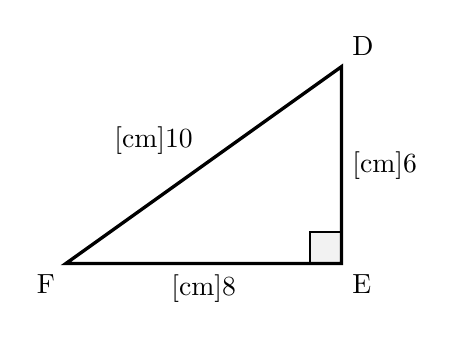
\begin{tikzpicture}[baseline={(0,1.25)}]
	\draw[line width=1pt, fill=gray!10] (3.1,0) rectangle ++(0.4,0.4) ;
	\draw[line width=1.2pt] (0,0)node[below left]{F}
	-- (3.5,2.5)node[above right]{D} node[pos=0.5,above left]{\np[cm]{10}}
	-- (3.5,0)node[below right]{E} node[pos=0.5,right]{\np[cm]{6}}
	-- cycle node[pos=0.5,below]{\np[cm]{8}};
\end{tikzpicture}
\end{center}

\needspace{25\baselineskip}
